\section{Results}
\label{sec:results}

Results are presented in the order in which they constrain the design: the grouping stage, the embedding network,
adaptation to real data, the end-to-end pipeline and its detector swap, the system-level view,
and the variants that did not improve on PG-GAT.
All values are pose grouping accuracy unless stated otherwise.

\subsection{Grouping heads against the $k$-means read-out}
\label{sec:results_heads}

% --- from chapter4_baseline.tex, chapter4_learned_heads.tex, chapter4_sa_dmon.tex ---
The grouping stage was tested as the bottleneck before any change to the embedding.
Three learned grouping heads were trained jointly with the standard two-layer GATv2 embedding under an identical schedule:
deep embedded clustering (DEC)~\citep{xie2016dec}, slot attention~\citep{locatello2020slotattention}
and supervised graph partitioning~\citep{yang2020gcnve}.
A skeleton-aware deep modularity network (SA-DMoN),
which adds pose structure to a modularity-based clustering objective~\citep{tsitsulin2023dmon},
was trained in ten variants under the same arrangement.
Table~\ref{tab:heads} compares all of them with $k$-means on the same kind of embedding.

\begin{table}[!t]
\centering
\caption{Learned grouping heads against the $k$-means read-out on the standard GATv2 embedding (two layers, $d=128$, synthetic training only).
COCO values use ground-truth keypoints.
``$k$-means'' clusters the embedding trained jointly with each head; ``head'' is the head's own read-out.}
\label{tab:heads}
\footnotesize\setlength{\tabcolsep}{3.5pt}
\begin{tabular}{lccc}
\toprule
Configuration & Synth val & COCO $k$-means & COCO head \\
\midrule
Standard GATv2 + $k$-means & 0.8783 & 0.8841 & --- \\
DEC & 0.8608 & 0.8798 & --- \\
Slot attention & 0.9025 & 0.8254 & 0.7986 \\
Graph partitioning & 0.9714 & 0.8366 & 0.7514 \\
SA-DMoN, 10 variants & 0.777--0.793 & 0.862--0.868 & 0.811--0.821 \\
\bottomrule
\end{tabular}
\end{table}

No head beats $k$-means once the models are scored on COCO.
Slot attention and graph partitioning raise synthetic accuracy, the latter by 0.0931,
but their own read-outs fall to 0.7986 and 0.7514 on COCO,
and $k$-means applied to their jointly trained embeddings still does better than the heads.
DEC leaves the representation largely untouched; its training target is built from its own soft assignments and supplies no identity information.
The ten SA-DMoN variants vary the spatial bandwidth, the null model, the adjacency, and the type loss,
yet all stay inside a 0.0165 band on synthetic data, the best of them 0.0849 below the baseline.
Adding capacity or structure after the embedding does not recover what the embedding lacks, which motivates building the structure into the embedding network itself.

\subsection{PG-GAT ablation and sweeps}
\label{sec:results_ablation}

% --- from chapter4_pggat_ablations.tex and chapter4_pggat_sweep.tex ---
Table~\ref{tab:ablation} isolates the three modifications, all run on the two-layer architecture
and synthetic-only schedule shared with the baseline.

\begin{table}[!t]
\centering
\caption{Isolation ablation of the three PG-GAT modifications at matched architecture (two layers, $d=128$) and training, synthetic training only.
COCO values use ground-truth keypoints.}
\label{tab:ablation}
\footnotesize\setlength{\tabcolsep}{3.5pt}
\begin{tabular}{lcc}
\toprule
Configuration & Synth val & COCO val \\
\midrule
Standard GATv2 (baseline) & 0.8783 & 0.8841 \\
Type-pair attention only & 0.8825 & 0.8819 \\
Position encoding only & 0.8825 & 0.8884 \\
Repulsion heads only & 0.8834 & 0.8785 \\
All three (PG-GAT) & 0.8896 & 0.8868 \\
\bottomrule
\end{tabular}
\end{table}

Each single modification lifts synthetic accuracy by between 0.0042 and 0.0051, and the three together add 0.0113,
a 0.0062 margin over the best single modification.
The single-modification values fall within 0.0009 of one another and are not read as a ranking:
each is a single run, and the individual margins sit close to the metric's run-to-run variation.
Zero-shot transfer to COCO is mixed.
Position encoding alone is the strongest configuration at 0.8884;
type-pair attention and repulsion alone fall slightly below the baseline;
and the full configuration lands 0.0027 above it.
The ablation supports retaining all three modifications but does not assign the later COCO gain to any single one.

The architecture sweep then lifts synthetic accuracy from 0.8896 to 0.9634 ---
a gain of 0.0738, the largest produced by any change to the embedding network ---
by selecting three layers and a 256-dimensional output.
The loss sweep finds no setting above the inherited one; its best run reaches 0.9617.
The benefit of the skeleton-aware modifications depends strongly on the capacity of the network that uses them.

\subsection{COCO fine-tuning}
\label{sec:results_finetune}

% --- from chapter4_coco_ft.tex ---
The architecture-sweep winner, trained on synthetic data only, transfers to COCO at 0.9010 on ground-truth keypoints;
Table~\ref{tab:finetune} records the effect of fine-tuning it on COCO.

\begin{table}[!t]
\centering
\caption{Effect of COCO fine-tuning on the architecture-sweep-selected PG-GAT.
COCO val groups ground-truth keypoints; COCO E2E groups HigherHRNet detections with the annotated person count.}
\label{tab:finetune}
\footnotesize\setlength{\tabcolsep}{3.5pt}
\begin{tabular}{lccc}
\toprule
Configuration & Synth val & COCO val & COCO E2E \\
\midrule
Synthetic only & 0.9634 & 0.9010 & 0.9005 \\
Earlier 20-epoch recipe$^{a}$ & 0.9178 & 0.9565 & 0.9430 \\
Single 20-epoch fine-tune & --- & 0.9695 & 0.9559 \\
Fine-tune sweep (final) & 0.9634 & 0.9715 & 0.9591 \\
\midrule
HigherHRNet AE (reference) & --- & --- & 0.9847 \\
\bottomrule
\end{tabular}

\smallskip
\footnotesize $^{a}$ applied to the two-layer PG-GAT of Table~\ref{tab:ablation}.
\end{table}

Fine-tuning is among the largest effects in the study: COCO accuracy rises by 0.0705 to 0.9715,
and end-to-end accuracy by 0.0586 to 0.9591.
The sweep over the fine-tuning recipe adds only 0.0020 on top of a single fine-tune;
this is not treated as a substantive gain, and its value lies in showing that the result does not depend on one narrowly chosen schedule.
Synthetic accuracy holds at 0.9634, and 0.9580 on the held-out synthetic test split; adaptation to COCO therefore does not come at the cost of the source domain.
On the 1\,248 images with at least two people, the final model reaches 0.9472.

\subsection{End-to-end grouping and detector swap}
\label{sec:results_e2e}

% --- from chapter4_e2e.tex 4.9.1-4.9.3 and 4.9.5 ---
Against the native AE grouping on the same matched HigherHRNet detections,
PG-GAT with the annotated person count reaches 0.9591 against 0.9847, a difference of 0.0256.
That same gap is 0.1081 for the synthetic-only two-layer PG-GAT,
0.0842 for the synthetic-only sweep-selected architecture,
0.0417 for the two-layer PG-GAT under the earlier fine-tuning recipe, and 0.0256 for the final model.
It is not a pure read-out of the cost of modularity: AE and PG-GAT also differ in representation, objective, and access to detector features.
It is, instead, the empirical gap between the modular pipeline and the detector's own grouping under a common protocol.

Swapping the annotated count for the K-head's prediction yields the autonomous pipeline, which consumes no ground truth at inference.
The K-head reproduces the exact annotated count in 76.1\,\% of the 2\,165 scenes and lands within one person in 91.9\,\%.
The autonomous pipeline reaches 0.9644, a 0.0053 margin over the pipeline given the annotated count.
Table~\ref{tab:swap} repeats the evaluation on the two further detectors, applying the same frozen PG-GAT
and K-head with no retraining, and Figure~\ref{fig:swap} shows one scene under all three.

\begin{table*}[!t]
\centering
\caption{Detector swap on COCO \texttt{val2017}.
Recall is the fraction of annotated keypoints matched by a detection within 10 pixels.
Native is each detector's own person assignment on its matched detections; the PG-GAT columns discard it
and re-group the pooled keypoints with the same frozen network,
using the annotated count or the K-head's prediction.
Gap is native minus autonomous PG-GAT; $\hat K$ gain is PG-GAT with $\hat K$ minus PG-GAT with the annotated $K$.
Scored images: 2\,165, 2\,196 and 2\,121.}
\label{tab:swap}
\footnotesize\setlength{\tabcolsep}{3.5pt}
\begin{tabular}{lcccccc}
\toprule
Detector (family) & Recall & Native & PG-GAT, $K$ & PG-GAT, $\hat K$ & Gap & $\hat K$ gain \\
\midrule
HigherHRNet-W32-512 (heatmaps and AE tags) & 0.793 & 0.9847 & 0.9591 & 0.9644 & 0.0203 & $+0.0053$ \\
YOLO11x-pose (single-stage regression) & 0.816 & 0.9863 & 0.9647 & 0.9653 & 0.0210 & $+0.0006$ \\
RTMO-L (one-stage bottom-up)$^{a}$ & 0.774 & 0.9961 & 0.9437 & 0.9741 & 0.0220 & $+0.0304$ \\
\bottomrule
\end{tabular}

\smallskip
\footnotesize $^{a}$ public \texttt{body7} weights, trained on a multi-dataset corpus rather than COCO alone.
\end{table*}

\begin{figure*}[!t]
    \centering
    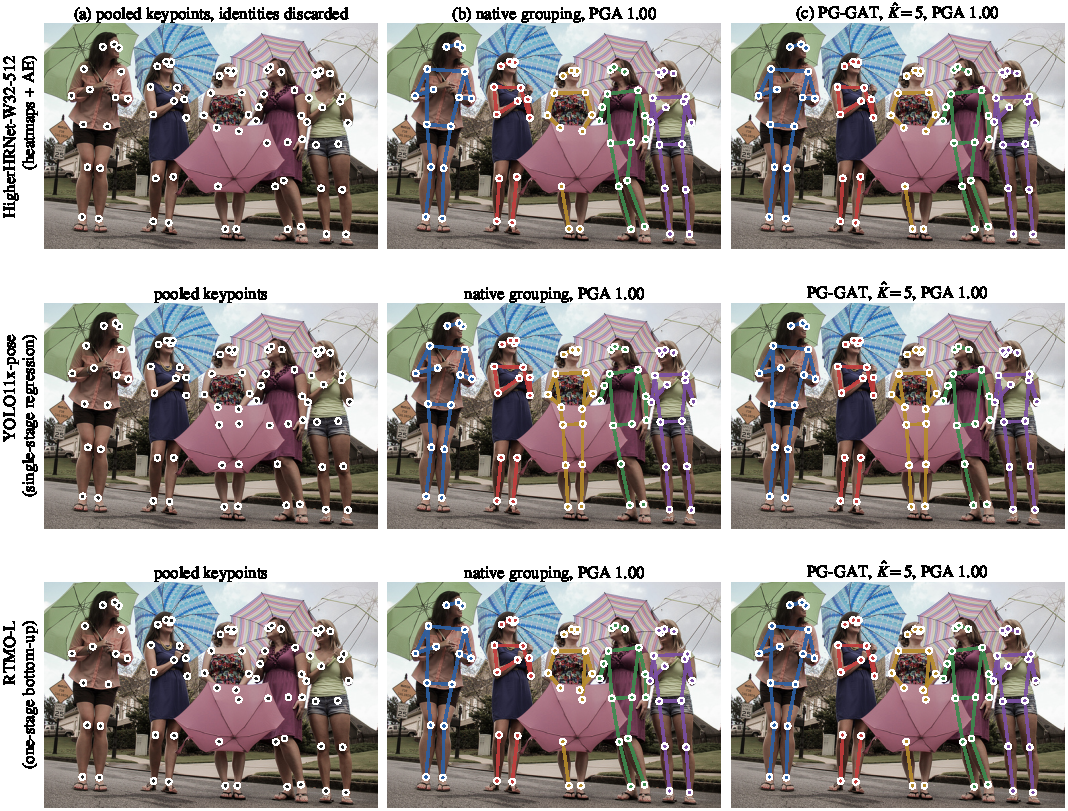
\includegraphics[width=\textwidth]{figures/detector_swap.pdf}
    \caption{One COCO \texttt{val2017} scene (281759, five people) under the three detectors,
    shown to illustrate reuse of the same frozen module rather than a typical error.
    (a) The detected keypoints with the detector's identities discarded, as they cross the interface.
    (b) The detector's native grouping.
    (c) The frozen PG-GAT grouping of all pooled detections with the predicted person count $\hat K$.
    Joints are drawn only where a detection is matched to ground truth and are coloured by the person their group maps to.
    All nine groupings of this scene are correct (accuracy 1.00), so every joint carries its own person's colour.}
    \label{fig:swap}
\end{figure*}

The autonomous pipeline trails the native grouping by 0.0203, 0.0210, and 0.0220 for the three detectors,
a 0.0017 spread across a heatmap-based bottom-up detector, a single-stage regression model,
and a one-stage bottom-up model whose native grouping comes from multi-dataset training.
The accuracy difference between the predicted and annotated counts also shifts systematically with the detector:
the predicted count is worth $+0.0006$ for YOLO11x-pose at a recall of 0.816,
$+0.0053$ for HigherHRNet at 0.793, and $+0.0304$ for RTMO-L at 0.774.
On ground-truth keypoints, where recall is complete, the predicted count instead costs 0.0066 against the annotated count.

\subsection{System-level average precision}
\label{sec:results_ap}

% --- from results.md "AP@OKS end-to-end (2026-09-09)" (not in the dissertation) ---
Table~\ref{tab:ap} scores the same HigherHRNet pipeline under AP@OKS on all 5\,000 \texttt{val2017} images,
with PG-GAT grouping every pooled detection, false positives included.

\begin{table}[!t]
\centering
\caption{AP@OKS on COCO \texttt{val2017} (5\,000 images) for HigherHRNet-W32-512 keypoints, single scale without flip.
All rows except the first group the same pooled joints (confidence above 0.1).}
\label{tab:ap}
\footnotesize\setlength{\tabcolsep}{3.5pt}
\begin{tabular}{lcccc}
\toprule
Grouping & AP & AP$_{50}$ & AP$_{75}$ & AR \\
\midrule
Native, full output & 0.583 & 0.769 & 0.638 & 0.677 \\
Native, pooled joints & 0.540 & 0.749 & 0.579 & 0.630 \\
PG-GAT, predicted $\hat K$ & 0.492 & 0.724 & 0.510 & 0.548 \\
PG-GAT, annotated $K$ & 0.483 & 0.719 & 0.503 & 0.537 \\
PG-GAT, detector's count & 0.484 & 0.713 & 0.503 & 0.539 \\
\bottomrule
\end{tabular}
\end{table}

On identical joints, the autonomous pipeline sits 0.048 AP below the native grouping,
and 0.116 below the native grouping's unrestricted output when both draw on every joint the detector returns (0.583 against 0.467).
The system-level cost is therefore larger than the grouping-level cost of about 0.02 measured on matched detections.
Figure~\ref{fig:crowd} splits both metrics by the number of annotated people.
The AP difference is 0.029 on images with one to five people and 0.076 on images with six or more,
the range beyond the person counts seen in synthetic training.
On matched detections the pose grouping accuracy gap grows in the same way, from 0.016 to 0.053.
At the protocol threshold the predicted count still outperforms the annotated count, 0.492 against 0.483 AP.

\begin{figure}[!t]
    \centering
    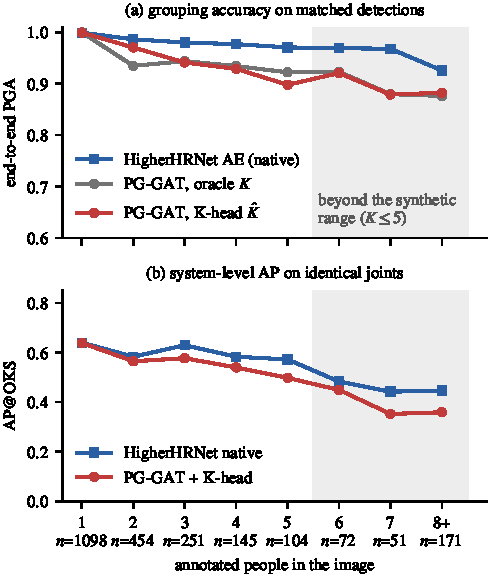
\includegraphics[width=\columnwidth]{figures/crowd_size.pdf}
    \caption{Performance by the number of annotated people in the image, HigherHRNet detections.
    (a) End-to-end pose grouping accuracy on matched detections.
    (b) AP@OKS on identical pooled joints.
    The shaded region lies beyond the person counts of the synthetic training data;
    $n$ is the number of images per bin in (b).}
    \label{fig:crowd}
\end{figure}

\subsection{Variants that did not improve on PG-GAT}
\label{sec:results_variants}

% --- from chapter4_hyperbolic.tex, chapter4_trigat.tex, chapter4_v2.tex ---
Each of three extensions tested a single assumption of the design; Table~\ref{tab:variants} summarises them.

\begin{table}[!t]
\centering
\caption{PG-GAT variants.
COCO val groups ground-truth keypoints; $d$ is the embedding dimension; v2 adds appearance features.}
\label{tab:variants}
\footnotesize\setlength{\tabcolsep}{3.5pt}
\begin{tabular}{lccc}
\toprule
Configuration & $d$ & Synth val & COCO val \\
\midrule
PG-GAT, two layers & 128 & 0.8896 & 0.8868 \\
Hyperbolic PG-GAT & 32 & 0.8856 & 0.8969 \\
TriGAT$^{a}$ & 128 & 0.8740 & 0.8564 \\
\midrule
PG-GAT, final & 256 & 0.9634 & 0.9715 \\
Hyperbolic, COCO fine-tuned & 32 & 0.8900 & 0.9399 \\
PG-GAT v2, 20 epochs & 128 & --- & 0.9670 \\
PG-GAT v2, 50 epochs & 128 & --- & 0.9682 \\
\bottomrule
\end{tabular}

\smallskip
\footnotesize $^{a}$ evaluated on the 2\,180 scenes with at least one valid triplet.
\end{table}

A hyperbolic output space on the Lorentz model~\citep{nickel2018lorentz},
chosen for the tree-like topology of the skeleton,
matches the 128-dimensional Euclidean model at 32 dimensions under synthetic training,
0.8856 against 0.8896.
Fine-tuning removes the advantage: the fine-tuned hyperbolic model reaches 0.9399 on COCO,
0.0316 below the final Euclidean model, and 0.9336 end to end.
TriGAT replaces joints with triplets of connected joints --- the pivot angle of a triplet describing local articulation independently of rotation ---
and votes the triplet clusters back onto joints; it lands 0.0156 below the matched PG-GAT on synthetic data
and 0.0304 below on COCO, with the loss traced to the voting stage.
PG-GAT v2 adds MobileNetV2 features~\citep{sandler2018mobilenetv2} sampled at each keypoint; it stays 0.0045
and 0.0033 below the final model while adding a further $2.2 \times 10^{6}$ frozen parameters at inference.
Because it extends the earlier two-layer architecture, it does not isolate the effect of appearance on the final configuration.
None of the three is a better operating point than the position-and-type PG-GAT.